Consider the following unity gain feedback system. Sketch a Nyquist plot when $K = 1$ and determine if the closed loop is stable. For full credit, the sketch should label important features like where the plot crosses the real or imaginary axes.
\begin{center}
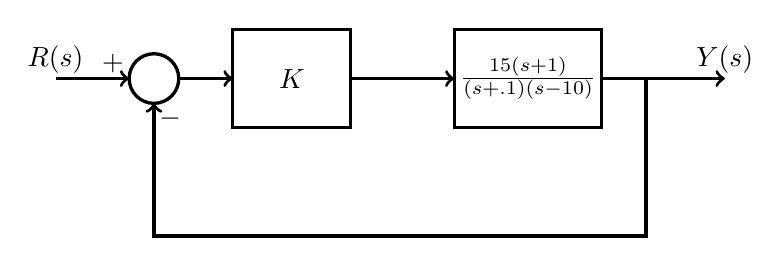
\begin{tikzpicture}[scale=1,inner sep=0pt,outer sep=0pt,very thick,
sysblock/.style={draw,rectangle,inner sep=2pt,minimum width=1.5cm,minimum height=1.25cm,very thick}]

\draw (1.25,0) node[draw,circle] (sum1) {$\rule{0pt}{18pt}$};
\draw (3,0) node[sysblock] (Kp) {$K$};
\draw (6,0) node[sysblock] (G) {$\frac{15(s+1)}{(s+.1)(s-10)}$};

\draw[->] (0,0) node[above=2pt] {$R(s)$} -- (sum1.180) node[above left=2pt] {$+$};
\draw[->] (sum1.0) --   (Kp);
\draw[->] (Kp) -- (G.180);
\draw[->] (G) -- ++(2.5,0) node[above=2pt] {$Y(s)$};
\draw[->] (G) ++(1.5,0) -- ++(0,-2) -| (sum1.-90) node[below right=2pt] {$-$};
\end{tikzpicture}
\end{center}
